\documentclass[spanish]{beamer}
\usepackage[utf8]{inputenc}
\usepackage{float}
\usepackage{beamerthemesplit}
\usepackage{latexsym}
\usepackage[T1]{fontenc}
\usepackage{amsmath}
\usepackage{hyperref}
\usepackage{graphicx}
\usepackage{babel,blindtext}
\usepackage{amsfonts}
\usepackage[round]{natbib}
\bibliographystyle{chicago}
\usepackage{subcaption} 
\usepackage{mathrsfs}


\decimalpoint

%\documentclass{beamer}
\usetheme[pageofpages=of,% String used between the current page and the
                         % total page count.
          bullet=circle,% Use circles instead of squares for bullets.
          titleline=true,% Show a line below the frame title.
          alternativetitlepage=true,% Use the fancy title page.
          titlepagelogo=logo,% Logo for the first page.
          watermark=logo2,% Watermark used in every page.
          watermarkheight=60px,% Height of the watermark.
          watermarkheightmult=3,% The watermark image is 4 times bigger
                                % than watermarkheight.
          ]{Torino}

%
%\usetheme{Antibes}%este es el templete que se usa a lo largo de la presentacion
%%themes
%%   default
%%   Boadilla
%%   Madrid
%%   Pittsburgh
%%   Copenhagen
%%   Warsaw
%%   Singapore
%%   Malmoe
%\newcommand\Fontvi{\fontsize{6}{7.2}\selectfont}
\mode<presentation>%tipo de 
\begin{document}

%%%%%%%%%%%%%%%%%%%%%%%%%%%%%%%%%%%%%%%%%%%%%%%%%%%%%%%%%%%%%%%%%%%%%%%%%%%%%%%%%%%%%%%%%%%%%%%%%%%%%%%%%%%%%
\title{Introduction}
\subtitle{Pattern Recognition}
\author{Gamaliel Moreno Chávez}
\institute{MCPI}
\date{Enero-Julio\\ 2021}%para que ponga la fecha de hoy 

\frame{\titlepage}
%%%%%%%%%%%%%%%%%%%%%%%%%%%%%%%%%%%%%%%%%%%%%%%%%%%%%%%%%%%%%%%%%%%%%%%%%%%%%%%%%%%%%%%%%%%%%%%%%%%%%%%%%%%%%
%%%%%%%%%%%%%%%%%%%%%%%%%%%%%%%%%%%%%%%%%%%%%%%%%%%%%%%%%%%%%%%%%%%%%%%%%%%%%%%%%%%%%%%%%%%%%%%%%%%%%%%%%%%%%%%%%%%%%%%%%%%%%%%%%%%%%%%%%%%%%%%%%%%%%%%%%%%%%%%%%%%%%%%%%%%%%%%%%%%%%%%%%%%%%%%%%%%%%%%%%%%%%%%%%%%%%%%%%%
%%%%%%%%%%%%%%%%%%%%%%%%%%%%%%%%%%%%%%%%%%%%%%%%%%%%%%%%%%%%%%%%%%%%%%%%%%%%%%%%%%%%%%%%%%%%%%%%%%%%%%%%%%%%%%%%%%%%%%%%%%%%%%%%%%%%%%%%%%%%%%%%%%%%%%%%%%%%%%%%%%%%%%%%%%%%%%%%%%%%%%%%%%%%%%%%%%%%%%%%%%%%%%%%%%%%%%%%%%

\begin{frame}
\frametitle{Introduction}
IS PATTERN RECOGNITION IMPORTANT?

Pattern recognition is the scientific discipline whose goal is the classification of
objects into a number of categories or classes. We will refer to these objects using the generic term patterns

\begin{itemize}
\item Machine vision
\item Character (letter or number) recognition
\item Computer-aided diagnosis
\item Speech recognition
\end{itemize}


\end{frame}

%%%%%%%%%%%%%%%%%%%%%%%%%%%%%%%%%%%%%%%%%%%%%%%%%%%%%%%%%%%%%%%%%%%%%%%%%%%%%%%%%%%%%%%%%%%%%%%%%%%%%%%%%%%%%
\begin{frame}
\frametitle{Introduction}
What is machine learning?

\begin{block}{Machine Learning or ML}
A computer program is said to learn from experience E with respect to some class of tasks T,
and performance measure P, if its performance at tasks in T, as measured by P, improves with
experience E.
\end{block}
we treat all unknown quantities (e.g., predictions about the future value of some quantity of interest, such as tomorrow’s temperature, or the parameters of some
model) as random variables, that are endowed with probability distributions which describe a weighted set of possible values the variable may have.
\end{frame}
%%%%%%%%%%%%%%%%%%%%%%%%%%%%%%%%%%%%%%%%%%%%%%%%%%%%%%%%%%%%%%%%%%%%%%%%%%%%%%%%%%%%%%%%%%%%%%%%%%%%%%%%%%%%%
\begin{frame}
\frametitle{Introduction}
Probabilistic modeling is the language used by most other areas of science and engineering

\begin{center}
\textit{Almost all of machine learning can be viewed in probabilistic terms, making probabilistic
thinking fundamental. It is, of course, not the only view. But it is through this view that we
can connect what we do in machine learning to every other computational science, whether that
be in stochastic optimization, control theory, operations research, econometrics, information
theory, statistical physics or bio-statistics. For this reason alone, mastery of probabilistic
thinking is essential.}
\end{center}
\end{frame}
%%%%%%%%%%%%%%%%%%%%%%%%%%%%%%%%%%%%%%%%%%%%%%%%%%%%%%%%%%%%%%%%%%%%%%%%%%%%%%%%%%%%%%%%%%%%%%%%%%%%%%%%%%%%%
\begin{frame}
\frametitle{Introduction}
Learning types: Supervised and Unsupervised learning
\begin{center}
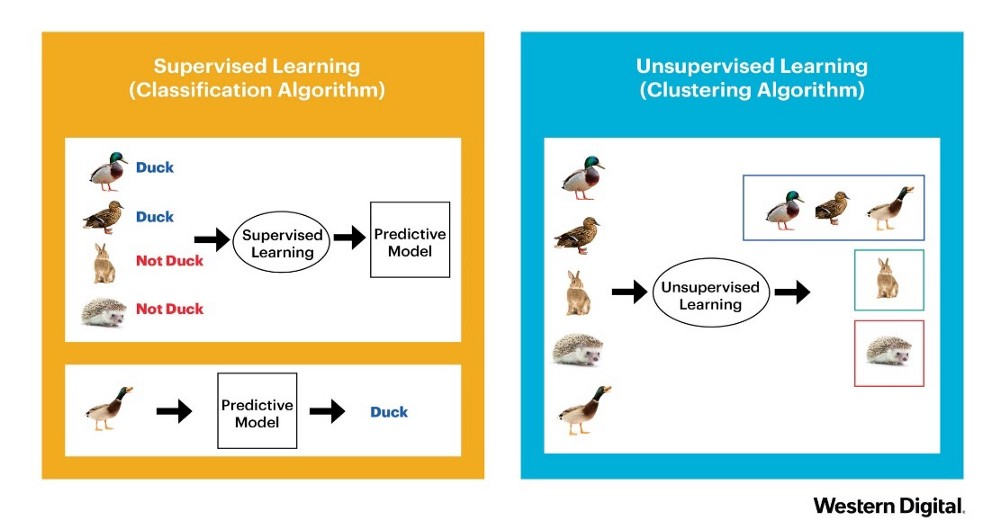
\includegraphics[scale=0.35]{im1}
\end{center}


\end{frame}
%%%%%%%%%%%%%%%%%%%%%%%%%%%%%%%%%%%%%%%%%%%%%%%%%%%%%%%%%%%%%%%%%%%%%%%%%%%%%%%%%%%%%%%%%%%%%%%%%%%%%%%%%%%%%
\begin{frame}
\frametitle{Introduction}
\textbf{Supervised learning}
\begin{itemize}
\item the task T is to learn a mapping $f$ from inputs $x \in X$ to outputs $y \in Y$.
\item The inputs x are also called the features, covariates, or predictors. This is often a fixed dimensional vector of numbers, such as the height
and weight of a person, or the pixels in an image.
\item $X = \mathbb{R}^{D}$, where $D$ is the dimensionality of the vector.
\item  The output $y$ is also known as the label, target, or response.
\item The experience $E$ is given in the form of a set of $N$ input-output pairs $ \mathcal{D} = \lbrace{(xn, yn)}\rbrace_{n=1}^{N}$ known as the training set.
\item $N$ is called the sample size.
\end{itemize} 

\end{frame}

%%%%%%%%%%%%%%%%%%%%%%%%%%%%%%%%%%%%%%%%%%%%%%%%%%%%%%%%%%%%%%%%%%%%%%%%%%%%%%%%%%%%%%%%%%%%%%%%%%%%%%%%%%%%%
\begin{frame}
\frametitle{Classification} 
In classification problems, the output space is a set of $C$ unordered and mutually exclusive labels
known as classes, $Y = \lbrace1, 2, \ldots ,C\rbrace$. The problem of predicting the class label given an input is
also called pattern recognition. If there are just two classes, often denoted by $y  \in \lbrace 0, 1\rbrace$ or
$y  \in \lbrace 0, 1\rbrace$, it is called binary classification.

\end{frame}
%%%%%%%%%%%%%%%%%%%%%%%%%%%%%%%%%%%%%%%%%%%%%%%%%%%%%%%%%%%%%%%%%%%%%%%%%%%%%%%%%%%%%%%%%%%%%%%%%%%%%%%%%%%%%
\begin{frame}
\frametitle{Classification}  
Example: classifying Iris flowers. Consider the problem of classifying iris flowers into their 3 subspecies, setosa, versicolor
and virginica.
\begin{center}
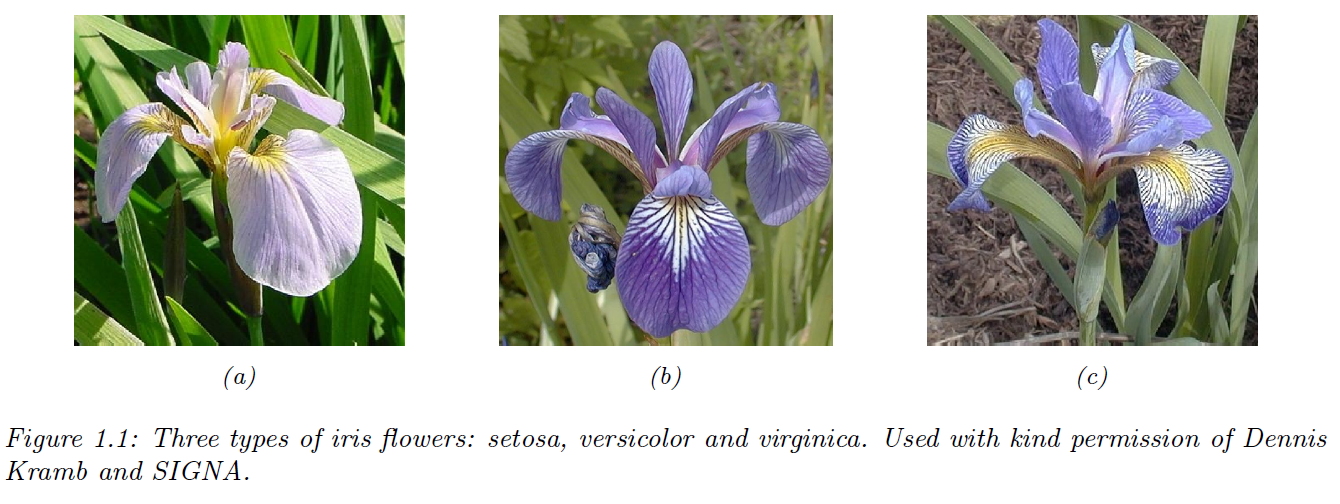
\includegraphics[width=\textwidth]{im2}
\end{center}
\end{frame}
%%%%%%%%%%%%%%%%%%%%%%%%%%%%%%%%%%%%%%%%%%%%%%%%%%%%%%%%%%%%%%%%%%%%%%%%%%%%%%%%%%%%%%%%%%%%%%%%%%%%%%%%%%%%%
\begin{frame}
\frametitle{Classification}  
Example: classifying Iris flowers. Consider the problem of classifying iris flowers into their 3 subspecies, setosa, versicolor
and virginica.
\begin{center}
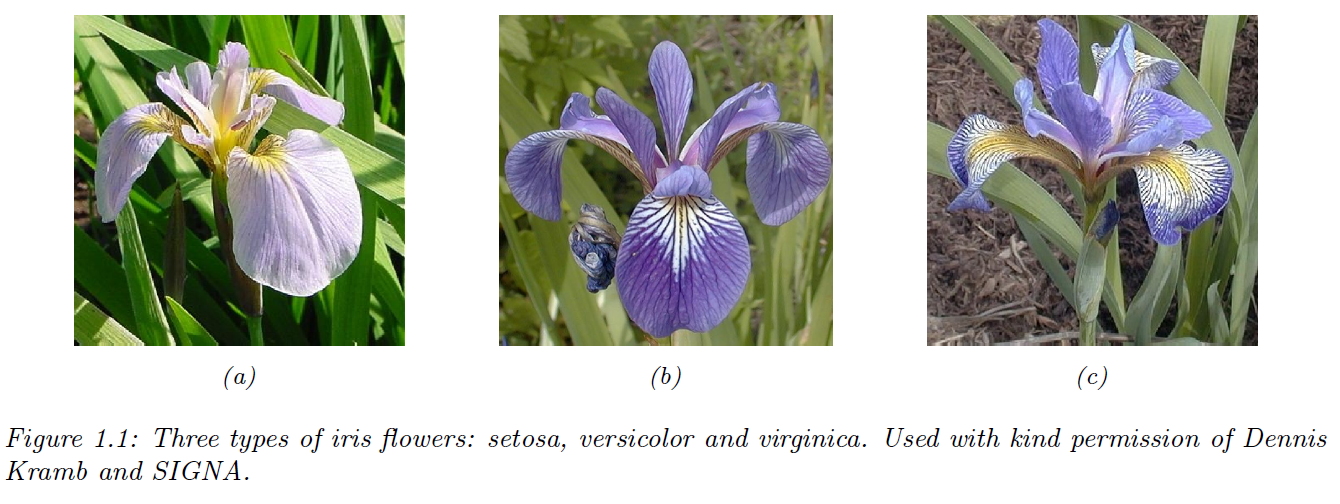
\includegraphics[width=\textwidth]{im2}
\end{center}
\end{frame}
%%%%%%%%%%%%%%%%%%%%%%%%%%%%%%%%%%%%%%%%%%%%%%%%%%%%%%%%%%%%%%%%%%%%%%%%%%%%%%%%%%%%%%%%%%%%%%%%%%%%%%%%%%%%%
\begin{frame}
\frametitle{Classification}  
In image classification, the input space $X$ is the set of images, which is a very high dimensional
space: for a color image with $C = 3$ channels (e.g., RGB) and $D_1 \times  D_2$ pixels, we have $X = \mathbb{R}^{D}$, where $D= C \times D_1 \times D_2$.

Some botanists have already identified 4 simple, but highly informative, numeric
feature: sepal length, sepal width, petal length, petal width

We will use this much lower dimensional input space,$X = \mathbb{R}^{D}$, for simplicity. The iris dataset is a collection of 150 labeled examples of iris flowers, 50 of
each type, described by these 4 features.
\end{frame}
%%%%%%%%%%%%%%%%%%%%%%%%%%%%%%%%%%%%%%%%%%%%%%%%%%%%%%%%%%%%%%%%%%%%%%%%%%%%%%%%%%%%%%%%%%%%%%%%%%%%%%%%%%%%%
\begin{frame}
\frametitle{Classification}  
It is common to store them in an $N\times D$ matrix, in which each row represents an example, and each column represents a feature. This is known as a design
matrix;
\begin{center}
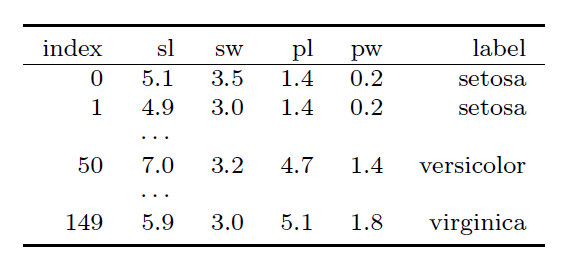
\includegraphics[width=\textwidth]{im3}
\end{center}

\end{frame}
%%%%%%%%%%%%%%%%%%%%%%%%%%%%%%%%%%%%%%%%%%%%%%%%%%%%%%%%%%%%%%%%%%%%%%%%%%%%%%%%%%%%%%%%%%%%%%%%%%%%%%%%%%%%%
\begin{frame}
\frametitle{Classification}  
Exploratory data analysis. Before tackling a problem with ML, it is usually a good idea to perform exploratory data analysis.

\begin{center}
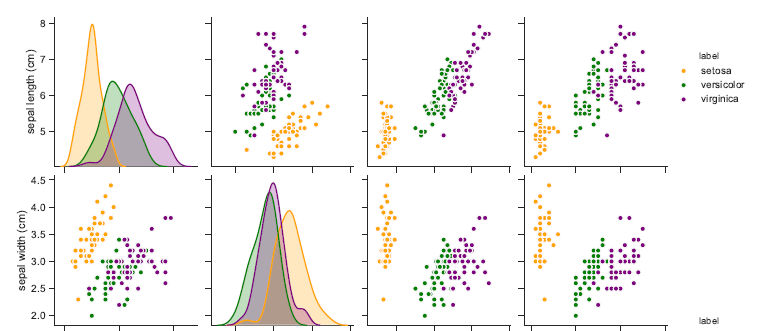
\includegraphics[width=\textwidth]{im4}
\end{center}

\end{frame}
%%%%%%%%%%%%%%%%%%%%%%%%%%%%%%%%%%%%%%%%%%%%%%%%%%%%%%%%%%%%%%%%%%%%%%%%%%%%%%%%%%%%%%%%%%%%%%%%%%%%%%%%%%%%%
\begin{frame}
\frametitle{Classification}  
Exploratory data analysis. Before tackling a problem with ML, it is usually a good idea to perform exploratory data analysis.

\begin{center}
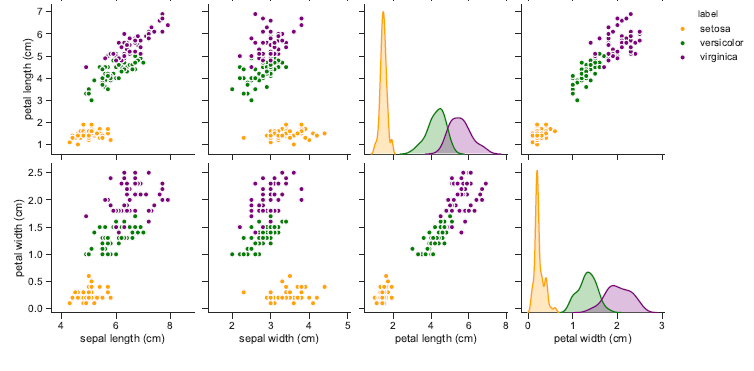
\includegraphics[width=\textwidth]{im5}
\end{center}

\end{frame}
%%%%%%%%%%%%%%%%%%%%%%%%%%%%%%%%%%%%%%%%%%%%%%%%%%%%%%%%%%%%%%%%%%%%%%%%%%%%%%%%%%%%%%%%%%%%%%%%%%%%%%%%%%%%%
\begin{frame}
\frametitle{Classification}  
We can see that the setosa class is easy to distinguish from the other two classes. For
example, suppose we create the following decision rule:

\begin{center}
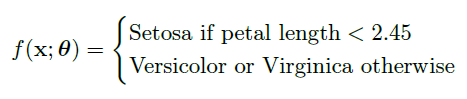
\includegraphics[width=\textwidth]{im6}
\end{center}
\end{frame}
%%%%%%%%%%%%%%%%%%%%%%%%%%%%%%%%%%%%%%%%%%%%%%%%%%%%%%%%%%%%%%%%%%%%%%%%%%%%%%%%%%%%%%%%%%%%%%%%%%%%%%%%%%%%%
\begin{frame}
\frametitle{Classification}  
We can arrange these nested rules in to a tree structure, \textbf{called a decision tree}.
\begin{center}
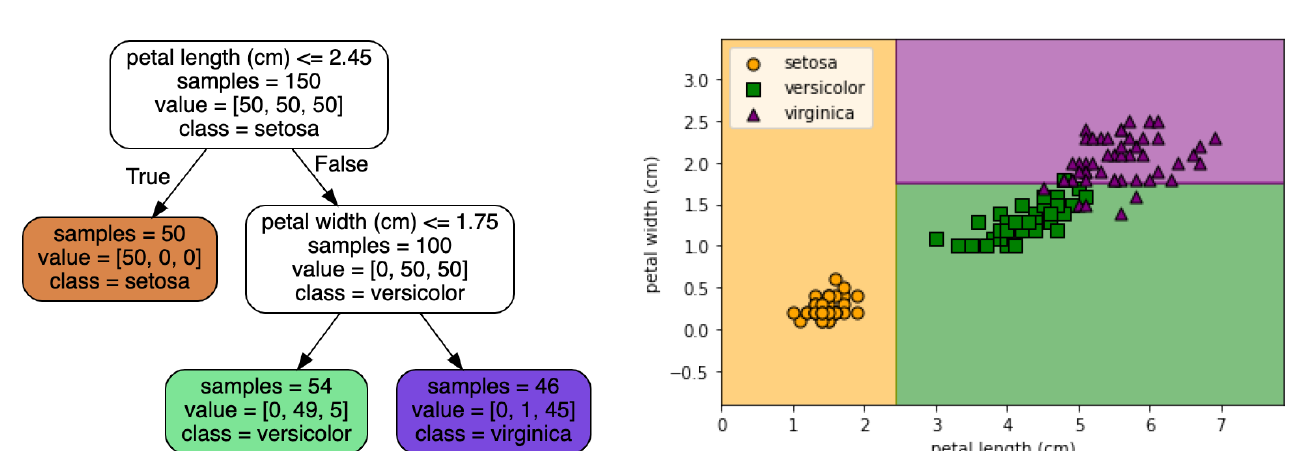
\includegraphics[width=\textwidth]{im7}
\end{center}
\end{frame}
%%%%%%%%%%%%%%%%%%%%%%%%%%%%%%%%%%%%%%%%%%%%%%%%%%%%%%%%%%%%%%%%%%%%%%%%%%%%%%%%%%%%%%%%%%%%%%%%%%%%%%%%%%%%%
\begin{frame}
\frametitle{Model fitting}
The goal of supervised learning is to automatically come up with classification models. A common way to
measure performance on this task is in terms of the misclassification rate on the training set:
\begin{equation*}
\mathcal{L}(\mathbf{\theta}) \triangleq \frac{1}{N} \sum_{n=1}^{N}{\mathbb{I}(y_{n}\neq f(x_{n};\mathbf{\theta})) }
\end{equation*}
where $\mathbb{I}(e)$ is the binary indicator function,
\begin{center}
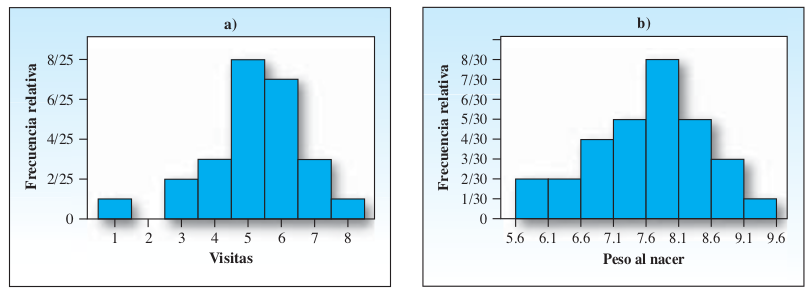
\includegraphics[scale=0.5]{im8}
\end{center}
\end{frame}
%%%%%%%%%%%%%%%%%%%%%%%%%%%%%%%%%%%%%%%%%%%%%%%%%%%%%%%%%%%%%%%%%%%%%%%%%%%%%%%%%%%%%%%%%%%%%%%%%%%%%%%%%%%%%
\begin{frame}
\frametitle{Model fitting}
For example, suppose we are foraging in the wilderness and we find some iris flowers.
Furthermore, suppose that setosa and versicolor are tasty, but virginica is poisonous. In this case, we
might use the asymmetric loss function
\begin{center}
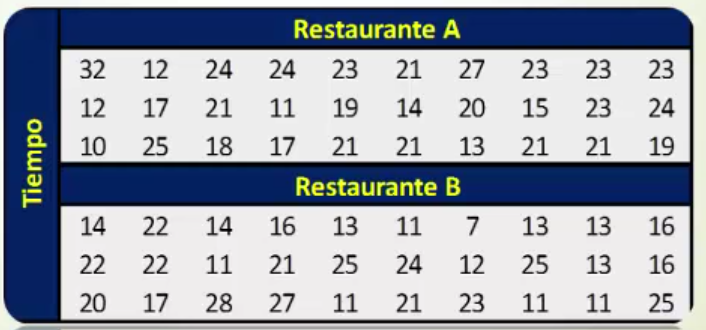
\includegraphics[scale=0.4]{im9}
\end{center}
\end{frame}
%%%%%%%%%%%%%%%%%%%%%%%%%%%%%%%%%%%%%%%%%%%%%%%%%%%%%%%%%%%%%%%%%%%%%%%%%%%%%%%%%%%%%%%%%%%%%%%%%%%%%%%%%%%%%
\begin{frame}
\frametitle{Model fitting}
We can then define empirical risk to be the average loss of the predictor on the training set:
\begin{equation*}
\mathcal{L}(\mathbf{\theta}) \triangleq \frac{1}{N} \sum_{n=1}^{N}{\ell(y_{n}, f(x_{n};\mathbf{\theta})) }
\end{equation*}
the empirical risk is equal to misclassification rate when we use zero-one loss for comparing the true label with the prediction
\begin{equation*}
\ell_{01}(y,\hat{y})= \mathbb{I}(y_{n}\neq \hat{y}) 
\end{equation*} 

\end{frame}
%%%%%%%%%%%%%%%%%%%%%%%%%%%%%%%%%%%%%%%%%%%%%%%%%%%%%%%%%%%%%%%%%%%%%%%%%%%%%%%%%%%%%%%%%%%%%%%%%%%%%%%%%%%%%
\begin{frame}
\frametitle{Model fitting}
One way to define the problem of model fitting or training is to find a setting of the parameters
that minimizes the empirical risk on the training set:
\begin{equation*}
\hat{\theta} =  \arg\min_{\theta} \mathcal{L}(\mathbf{\theta})  =\arg\min_{\theta} \frac{1}{N} \sum_{n=1}^{N}{l(y_{n}, f(x_{n};\mathbf{\theta})) }
\end{equation*}
This is called empirical risk minimization.
\end{frame}

%%%%%%%%%%%%%%%%%%%%%%%%%%%%%%%%%%%%%%%%%%%%%%%%%%%%%%%%%%%%%%%%%%%%%%%%%%%%%%%%%%%%%%%%%%%%%%%%%%%%%%%%%%%%%
\begin{frame}
\frametitle{Uncertainty}
In many cases, we will not be able to perfectly predict the exact output given the input, due to
lack of knowledge of the input-output mapping (this is called epistemic uncertainty or model
uncertainty), and/or due to intrinisic (irreducible) stochasticity in the mapping (this is called
aleatoric uncertainty or data uncertainty).We can capture our uncertainty using the following conditional
probability distribution:
%
\begin{equation*}
p(y=c\vert x ; \theta)=f_{c}(x; \theta)
\end{equation*}


where $f:X\rightarrow [0; 1]^C$ maps inputs to a probability distribution over the C possible output labels.
\end{frame}

%%%%%%%%%%%%%%%%%%%%%%%%%%%%%%%%%%%%%%%%%%%%%%%%%%%%%%%%%%%%%%%%%%%%%%%%%%%%%%%%%%%%%%%%%%%%%%%%%%%%%%%%%%%%%
\begin{frame}
\frametitle{Uncertainty}
When fitting probabilistic models, it is common to use the negative log probability as our loss
function:
\begin{equation*}
\ell(y,f(x;\theta))= -log p(y\vert f(x;\theta) )
\end{equation*}
The reasons for this are explained after, but the intuition is that a good model (with low
loss) is one that assigns a high probability to the true output y for each corresponding input x. The
average negative log probability of the training set is given by
\begin{equation*}
NNL(\theta)= \frac{1}{N}\sum_{n=1}^{N} log p(y\vert f(x;\theta) )
\end{equation*}
This is called the \textbf{negative log likelihood}.
\end{frame}


%%%%%%%%%%%%%%%%%%%%%%%%%%%%%%%%%%%%%%%%%%%%%%%%%%%%%%%%%%%%%%%%%%%%%%%%%%%%%%%%%%%%%%%%%%%%%%%%%%%%%%%%%%%%%
\begin{frame}
\frametitle{Regression}
Now suppose that we want to predict a real-valued quantity $y\in \mathfrak{R}$ instead of a class label $y\in \lbrace 1, \ldots,C \rbrace$
this is known as regression. For example, in the case of Iris flowers, $y$ might be the degree of toxicity if the flower is eaten, or the average height of the plant.
Regression is very similar to classification. However, since the output is real-valued, we need to
use a different loss function. For regression, the most common choice is to use quadratic loss, or $l_{2}$
loss:
\begin{equation*}
\ell_{2}(y, \hat{y})=(y-\hat{y})^2
\end{equation*}


\end{frame}
%%%%%%%%%%%%%%%%%%%%%%%%%%%%%%%%%%%%%%%%%%%%%%%%%%%%%%%%%%%%%%%%%%%%%%%%%%%%%%%%%%%%%%%%%%%%%%%%%%%%%%%%%%%%%
\begin{frame}
\frametitle{Linear regression}
We can fit this data using a simple linear regression model of the form

\begin{equation*}
f(x;\theta)=b+wx 
\end{equation*}
\begin{center}
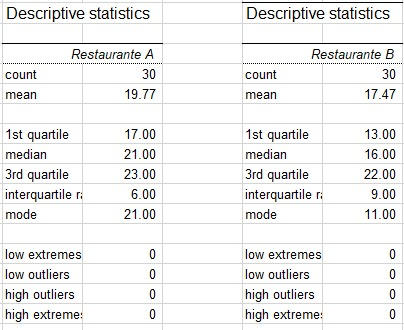
\includegraphics[scale=0.4]{im10}
\end{center}

where $w$ is the slope, $b$ is the offset, and $\theta= (w,b)$ are all the parameters of the model. 

\end{frame}
%%%%%%%%%%%%%%%%%%%%%%%%%%%%%%%%%%%%%%%%%%%%%%%%%%%%%%%%%%%%%%%%%%%%%%%%%%%%%%%%%%%%%%%%%%%%%%%%%%%%%%%%%%%%%
\begin{frame}
\frametitle{Linear regression}
By adjusting, we can minimize the sum of squared errors until we find the least squares solution

\begin{equation*}
\hat{\theta}= \arg\min_{\theta} MSE(\theta)
\end{equation*}

If we have multiple input features, we can write

\begin{equation*}
f(x;\theta) = b + w_{1}x_{1} +\cdots+ w_{D}x_{D} = b + \boldsymbol {w}^{T}\boldsymbol {x}
\end{equation*}
where$\boldsymbol {\theta}= (w; b)$. This is called \textbf{multiple linear regression}.
\end{frame}
%%%%%%%%%%%%%%%%%%%%%%%%%%%%%%%%%%%%%%%%%%%%%%%%%%%%%%%%%%%%%%%%%%%%%%%%%%%%%%%%%%%%%%%%%%%%%%%%%%%%%%%%%%%%%
\begin{frame}
\frametitle{Linear regression}
The fitted plane has the form $\hat{f}(\boldsymbol {x}) = w_0 + w_1x_1 + w_2x_2$.

\begin{center}
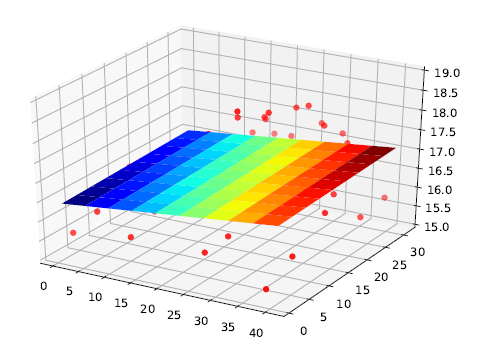
\includegraphics[width=0.8\textwidth]{im11}
\end{center}


\end{frame}
%%%%%%%%%%%%%%%%%%%%%%%%%%%%%%%%%%%%%%%%%%%%%%%%%%%%%%%%%%%%%%%%%%%%%%%%%%%%%%%%%%%%%%%%%%%%%%%%%%%%%%%%%%%%%
\begin{frame}
\frametitle{Linear regression}
 We can extend this model to use $D > 2$ input features (such as time of day), but then it becomes
harder to visualize. To reduce notational clutter, it is standard to absorb the bias term b into the weights $\boldsymbol {w}$ by defining
$\tilde{w} = [b,w_1, \ldots,wD]$ and defining $\tilde{x} = [1, x_1, \ldots, x_{D}]$, so that
\begin{equation*}
\tilde{w}^T  \tilde{x} = \boldsymbol{w}^T\boldsymbol{x}+ b
\end{equation*}
This converts the affine function into a linear function.
In statistics, the $ \boldsymbol{w}$ parameters are usually called regression coefficients (and are typically
denoted by $ \boldsymbol{ \beta}$) and $b$ is called the intercept. In ML, the parameters $\boldsymbol{w}$ are called the\textbf{ weights} and $b$
is called the \textbf{bias}.
\end{frame}
%%%%%%%%%%%%%%%%%%%%%%%%%%%%%%%%%%%%%%%%%%%%%%%%%%%%%%%%%%%%%%%%%%%%%%%%%%%%%%%%%%%%%%%%%%%%%%%%%%%%%%%%%%%%%
\begin{frame}
\frametitle{Polynomial regression}
We can improve the fit by using a \textbf{polynomial regression} model of degree D. This has the form $f(x;\boldsymbol{w}) = \boldsymbol{w}^T \phi(x)$, where $\phi(x)$ is a feature vector derived from the input, which has the following form:
\begin{equation*}
 \phi(x)=[1,x,x^2,\ldots,x^D]
\end{equation*}
we see that using $D = 2$ results in a much better fit. We can keep increasing $D$, and
hence the number of parameters in the model, until $D = N-1$; in this case, we have one parameter per data point, so we can perfectly interpolate the data. The resulting model will have 0 MSE. However, intuitively the resulting function will not be a good predictor for future
inputs, since it is too “wiggly”.
\end{frame}
%%%%%%%%%%%%%%%%%%%%%%%%%%%%%%%%%%%%%%%%%%%%%%%%%%%%%%%%%%%%%%%%%%%%%%%%%%%%%%%%%%%%%%%%%%%%%%%%%%%%%%%%%%%%%
\begin{frame}
\frametitle{Polynomial regression}

\begin{center}
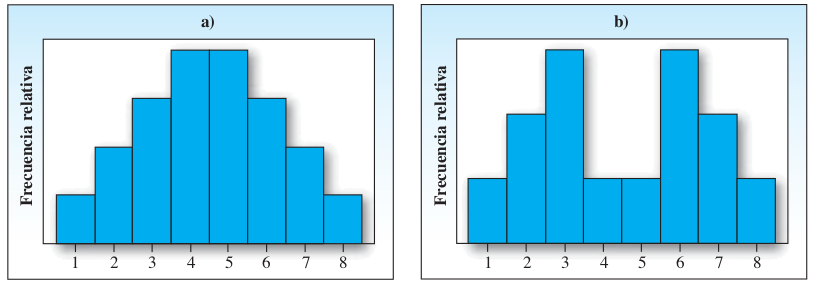
\includegraphics[width=0.6\textwidth]{im12}
\end{center}

\end{frame}
%%%%%%%%%%%%%%%%%%%%%%%%%%%%%%%%%%%%%%%%%%%%%%%%%%%%%%%%%%%%%%%%%%%%%%%%%%%%%%%%%%%%%%%%%%%%%%%%%%%%%%%%%%%%%
\begin{frame}
\frametitle{Polynomial regression}
We can also apply polynomial regression to multi-dimensional inputs.For example, next figure plots the predictions for the temperature model after performing a quadratic expansion of the inputs
\begin{center}
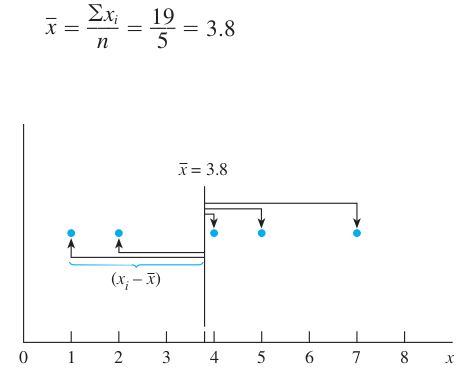
\includegraphics[width=0.5\textwidth]{im13}
\end{center}
We can also add cross terms, such as $x_1 x_2$, to capture
interaction effects.
\end{frame}
%%%%%%%%%%%%%%%%%%%%%%%%%%%%%%%%%%%%%%%%%%%%%%%%%%%%%%%%%%%%%%%%%%%%%%%%%%%%%%%%%%%%%%%%%%%%%%%%%%%%%%%%%%%%%
\begin{frame}
\frametitle{Deep neural networks}
We can create much more powerful models by learning  to do such nonlinear feature extraction automatically. If we let $ \phi(x)$ have its own set of parameters,
say $\boldsymbol{V}$, then the overall model has the form

\begin{equation*}
f(x;w,\boldsymbol{V})= w^T \phi(x;\boldsymbol{V})
\end{equation*}
%We can recursively decompose the feature extractor $\phi(x;\boldsymbol{V})$ into a composition of simpler functions.
The resulting model then becomes a stack of L nested functions:
\begin{equation*}
f(x;\boldsymbol{\theta})= f_{L}(f_{L-1}(\cdots (f_{1}(x)) \cdots))
\end{equation*}

where $f_{\ell}(x) = f(x;\theta_{\ell})$ is the function at layer $\ell$. The final layer is linear and has the form

$f_{L}(x) = w^T f_{1:L-1}(x)$, where $f_{1:L-1}(x)$ is the learned feature extractor. This is the key idea behind
\textbf{deep neural networks} or \textbf{DNNs}.

\end{frame}
%%%%%%%%%%%%%%%%%%%%%%%%%%%%%%%%%%%%%%%%%%%%%%%%%%%%%%%%%%%%%%%%%%%%%%%%%%%%%%%%%%%%%%%%%%%%%%%%%%%%%%%%%%%%%
\begin{frame}
\frametitle{Overfitting and generalization}
We can rewrite the empirical risk in the following equivalent way:

\begin{equation*}
\mathcal{L}(\mathbf{\theta}; \mathcal{D}_{train})= \frac{1}{\vert \mathcal{D}_{train}\vert }  \sum_{(x_n,y_n)\in \mathcal{D}_{train}  } \ell (y_{n}, f(x_{n});\boldsymbol{\theta})
\end{equation*}
where $N = \vert Dtrain \vert$ is the size of the training set $ \mathcal{D}_{train}$. This formulation is useful because it makes
explicit which dataset the loss is being evaluated on.

 A model that perfectly fits the training data, but which is too complex, is said to suffer from \textbf{overfitting}.

\end{frame}
%%%%%%%%%%%%%%%%%%%%%%%%%%%%%%%%%%%%%%%%%%%%%%%%%%%%%%%%%%%%%%%%%%%%%%%%%%%%%%%%%%%%%%%%%%%%%%%%%%%%%%%%%%%%%
\begin{frame}
\frametitle{Overfitting and generalization}

\begin{center}
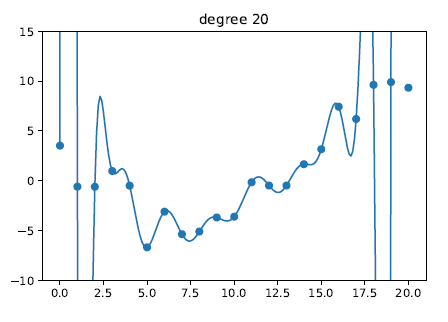
\includegraphics[scale=0.4]{im14}
\end{center}
To detect if a model is overfitting, let us assume (for now) that we have access to the true (but
unknown) distribution $p*(x; y)$ used to generate the training set. Then, instead of computing the
empirical risk we compute the theoretical expected loss or \textbf{population risk}
\begin{equation}
\mathcal{L}(\boldsymbol{\theta} ;P) \triangleq \mathbf{E}_{p*(x,y)}[\ell(y,f(x;\boldsymbol{\theta} ))]
\end{equation}

\end{frame}
%%%%%%%%%%%%%%%%%%%%%%%%%%%%%%%%%%%%%%%%%%%%%%%%%%%%%%%%%%%%%%%%%%%%%%%%%%%%%%%%%%%%%%%%%%%%%%%%%%%%%%%%%%%%%
\begin{frame}
\frametitle{Overfitting and generalization}
In practice we don’t know $p*$. However, we can partition the data we do have into two subsets,
known as the training set and the \textbf{test set}. Then we can approximate the population risk using the
\textbf{test risk}

\begin{equation*}
\mathcal{L}(\mathbf{\theta}; \mathcal{D}_{test})= \frac{1}{\vert \mathcal{D}_{test} \vert }  \sum_{(x_n,y_n)\in \mathcal{D}_{test}  } \ell (y_{n}, f(x_{n}) 
\end{equation*}
In practice, we need to partition the data into three sets, namely the training set, the test set and
a validation set; the latter is used for model selection, and we just use the test set to estimate
future performance (the population risk), i.e., the test set is not used for model fitting or model
selection.

\end{frame}
%%%%%%%%%%%%%%%%%%%%%%%%%%%%%%%%%%%%%%%%%%%%%%%%%%%%%%%%%%%%%%%%%%%%%%%%%%%%%%%%%%%%%%%%%%%%%%%%%%%%%%%%%%%%%
\begin{frame}
\frametitle{No free lunch theorem}
\begin{block}{No free lunch theorem}
There is no single best model that works optimally for all kinds of problems — this
is sometimes called the no free lunch theorem \footnote{ D. Wolpert. “The lack of a priori distinctions
between learning algorithms”. In: Neural Computation
8.7 (1996), pp. 1341–1390 (page 12).}.
\end{block}
For this reason, it is important to have many models and algorithmic techniques in one’s toolbox to choose
from.


\end{frame}
%%%%%%%%%%%%%%%%%%%%%%%%%%%%%%%%%%%%%%%%%%%%%%%%%%%%%%%%%%%%%%%%%%%%%%%%%%%%%%%%%%%%%%%%%%%%%%%%%%%%%%%%%%%%%
\begin{frame}
\frametitle{Unsupervised learning}
An arguably much more interesting task is to try to “make sense of” data, as opposed to just
learning a mapping. That is, we just get observed “inputs” $ \mathcal{D}  = \lbrace x_n : n = 1 : N\rbrace$ without any
corresponding “outputs” $y_{n}$. This is called \textbf{unsupervised learning}.


From a probabilistic perspective, we can view the task of unsupervised learning as fitting an
unconditional model of the form $p(x)$.
\end{frame}

%%%%%%%%%%%%%%%%%%%%%%%%%%%%%%%%%%%%%%%%%%%%%%%%%%%%%%%%%%%%%%%%%%%%%%%%%%%%%%%%%%%%%%%%%%%%%%%%%%%%%%%%%%%%%
\begin{frame}
\frametitle{Unsupervised learning}
\begin{itemize}
\item Unsupervised learning avoids the need to collect large labeled datasets for training
\item Unsupervised learning also avoids the need to learn how to partition the world into often arbitrary
categories.
\item Finally, unsupervised learning forces the model to “explain” the high dimensional inputs
\end{itemize}

\end{frame}
%%%%%%%%%%%%%%%%%%%%%%%%%%%%%%%%%%%%%%%%%%%%%%%%%%%%%%%%%%%%%%%%%%%%%%%%%%%%%%%%%%%%%%%%%%%%%%%%%%%%%%%%%%%%%
\begin{frame}
\frametitle{Clustering}
A simple example of unsupervised learning is the problem of finding clusters in data. The goal is to
partition the input into regions that contain “similar” points.
\begin{center}
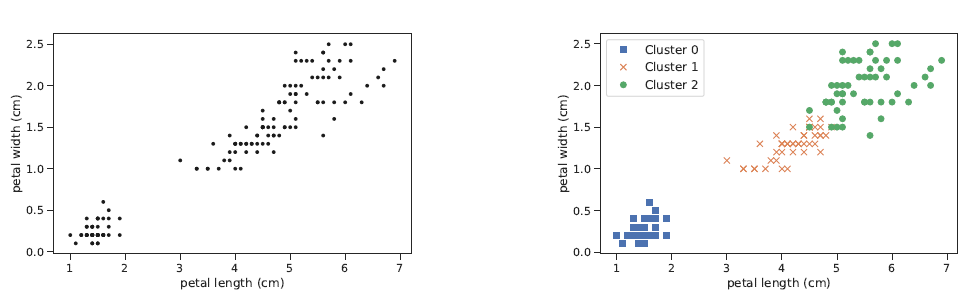
\includegraphics[scale=0.4]{im15}
\end{center}

\end{frame}
%%%%%%%%%%%%%%%%%%%%%%%%%%%%%%%%%%%%%%%%%%%%%%%%%%%%%%%%%%%%%%%%%%%%%%%%%%%%%%%%%%%%%%%%%%%%%%%%%%%%%%%%%%%%%
\begin{frame}
\frametitle{Self-supervised learning}

A recently popular approach to unsupervised learning is known as self-supervised learning. In
this approach, we create proxy supervised tasks from unlabeled data.For example, we might try to learn to predict a color image from a gray scale image, or to mask out words in a sentence and then try to predict them given the surrounding context. The hope is that the resulting predictor
$\hat{x}_1=f(x_2;\mathbf{\theta}$), where $x_2$ is the observed input and $x_1$ is the predicted output, will learn useful
features from the data, that can then be used in standard, downstream supervised tasks.

\end{frame}
%%%%%%%%%%%%%%%%%%%%%%%%%%%%%%%%%%%%%%%%%%%%%%%%%%%%%%%%%%%%%%%%%%%%%%%%%%%%%%%%%%%%%%%%%%%%%%%%%%%%%%%%%%%%%
\begin{frame}
\frametitle{Evaluating unsupervised learning}
it is very hard to evaluate the quality of the output of
an unsupervised learning method, because there is no ground truth to compare. A common method for evaluating unsupervised models is to measure the probability assigned by the model to unseen test examples. We can do this by computing the (unconditional) negative log likelihood of the data: 
\begin{equation*}
\mathcal{L}(\mathbf{\theta}; \mathcal{D})= \frac{1}{\vert \mathcal{D} \vert } \sum_{(x\in \mathcal{D} ) }log\text{ } p(x\vert \mathbf{\theta}) 
\end{equation*}
This treats the problem of unsupervised learning as one of density estimation.                                                                                

\end{frame}
%%%%%%%%%%%%%%%%%%%%%%%%%%%%%%%%%%%%%%%%%%%%%%%%%%%%%%%%%%%%%%%%%%%%%%%%%%%%%%%%%%%%%%%%%%%%%%%%%%%%%%%%%%%%%
\begin{frame}
\frametitle{Reinforcement learning}
addition to supervised and unsupervised learning, there is a third kind of ML known as \textbf{reinforcement learning} (RL). In this class of problems, the system or agent has to learn how to interact with its environment. This can be encoded by means of a policy $a =\pi(x)$, which specifies which action to take in response to each possible input $x$ (derived from the environment state).

\begin{block}{Definición}
El \textbf{puntaje z muestral} es una medida de posición relativa definida
por
\begin{equation*}
\text{puntaje } z = \frac{x-\bar{x}}{s}
\end{equation*}
\end{block}

Un puntaje z mide la distancia entre una observación y la media, medidas en unidades de desviación estándar.

\end{frame}
%%%%%%%%%%%%%%%%%%%%%%%%%%%%%%%%%%%%%%%%%%%%%%%%%%%%%%%%%%%%%%%%%%%%%%%%%%%%%%%%%%%%%%%%%%%%%%%%%%%%%%%%%%%%%
\begin{frame}
\frametitle{Mediciones de posición relativa }
Por ejemplo, suponga que la media y desviación estándar de los puntajes de examen (basados en un total de 35 puntos) son 25 y 4, respectivamente. El puntaje z para una calificación de 30 se calcula como sigue:

\begin{equation*}
\text{puntaje } z = \frac{x-\bar{x}}{s}=\frac{30-25}{4}=1.25
\end{equation*}

El puntaje de 30 está a 1.25 desviaciones estándar arriba de la media $(30 = \bar{x}+1.25s)$.
\end{frame}
%%%%%%%%%%%%%%%%%%%%%%%%%%%%%%%%%%%%%%%%%%%%%%%%%%%%%%%%%%%%%%%%%%%%%%%%%%%%%%%%%%%%%%%%%%%%%%%%%%%%%%%%%%%%%
\begin{frame}
\frametitle{Mediciones de posición relativa }
\begin{center}
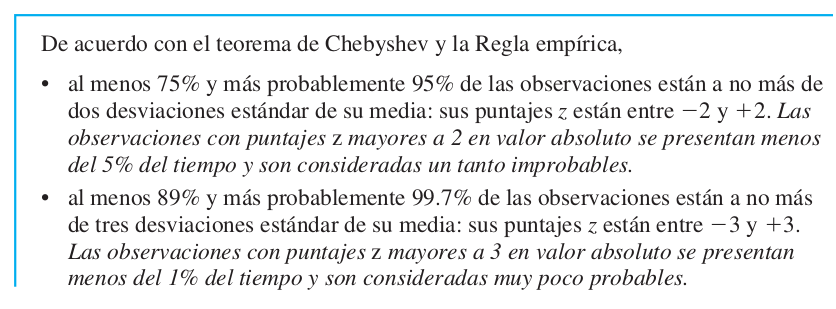
\includegraphics[scale=0.4]{im24}
\end{center}
\end{frame}
%%%%%%%%%%%%%%%%%%%%%%%%%%%%%%%%%%%%%%%%%%%%%%%%%%%%%%%%%%%%%%%%%%%%%%%%%%%%%%%%%%%%%%%%%%%%%%%%%%%%%%%%%%%%%
\begin{frame}
\frametitle{Percentil}
Un percentil es otra medida de posición relativa y se usa con más frecuencia para conjuntos grandes de datos. (Los percentiles no son muy útiles para conjuntos pequeños de datos).

\begin{block}{Definición}
Un conjunto de n mediciones de la variable $x$ se ha reacomodado en
orden de magnitud. El p-ésimo percentil es el valor de $x$ que es mayor a $p\%$ de las mediciones y es menor que el restante $(100 - p)\%$.
\end{block}


\end{frame}
%%%%%%%%%%%%%%%%%%%%%%%%%%%%%%%%%%%%%%%%%%%%%%%%%%%%%%%%%%%%%%%%%%%%%%%%%%%%%%%%%%%%%%%%%%%%%%%%%%%%%%%%%%%%%
\begin{frame}
\frametitle{Percentil}
Supongamos que usted ha sido notificado que su calificación de 610, en el Examen verbal de graduación, lo ha colocado en el 60avo percentil en la distribución de calificaciones. ¿Dónde está su calificación de 610 en relación a las calificaciones de los otros que tomaron el examen?

\vspace{1em}
Solución Calificar en el 60avo percentil significa que $60\%$ de todas las calificaciones de examen fueron más bajas que la calificación de usted y $40\%$ fueron más altas.

\end{frame}
%%%%%%%%%%%%%%%%%%%%%%%%%%%%%%%%%%%%%%%%%%%%%%%%%%%%%%%%%%%%%%%%%%%%%%%%%%%%%%%%%%%%%%%%%%%%%%%%%%%%%%%%%%%%%
\begin{frame}
\frametitle{Percentil}
En general, el 60avo percentil para la variable x es un punto en el eje horizontal de la distribución de datos que es mayor a 60\% de las mediciones y menor que las otras.

\begin{center}
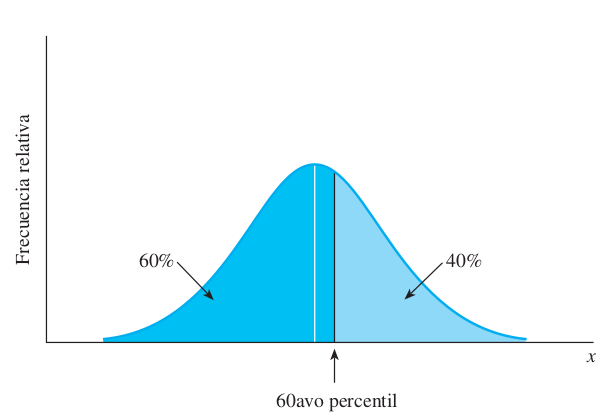
\includegraphics[scale=0.4]{im25}
\end{center}

\end{frame}
%%%%%%%%%%%%%%%%%%%%%%%%%%%%%%%%%%%%%%%%%%%%%%%%%%%%%%%%%%%%%%%%%%%%%%%%%%%%%%%%%%%%%%%%%%%%%%%%%%%%%%%%%%%%%
\begin{frame}
\frametitle{Percentil-Cuartil}

\begin{itemize}
\item La mediana es igual que el 50avo percentil.
\item Los percentiles 25avo y 75avo, llamados cuartiles inferior y superior
\item Veinticinco por ciento de las mediciones serán menores que el cuartil inferior (primero).
\item 50\% serán menores que la mediana (el segundo cuartil).
\item 75\% serán menores que el cuartil superior (tercero).
\end{itemize}

\end{frame}
%%%%%%%%%%%%%%%%%%%%%%%%%%%%%%%%%%%%%%%%%%%%%%%%%%%%%%%%%%%%%%%%%%%%%%%%%%%%%%%%%%%%%%%%%%%%%%%%%%%%%%%%%%%%%
\begin{frame}
\frametitle{Cuartil}

\begin{center}
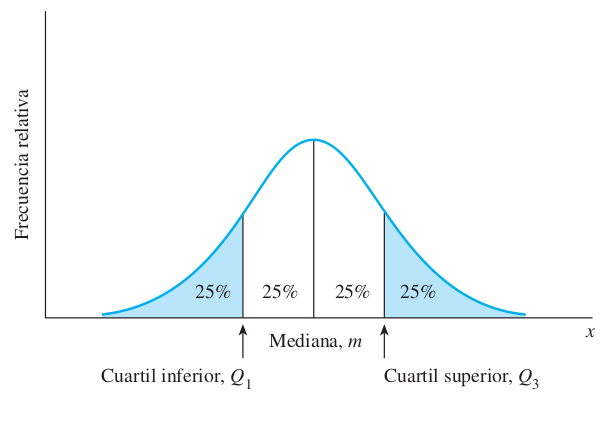
\includegraphics[scale=0.4]{im26}
\end{center}

\end{frame}
%%%%%%%%%%%%%%%%%%%%%%%%%%%%%%%%%%%%%%%%%%%%%%%%%%%%%%%%%%%%%%%%%%%%%%%%%%%%%%%%%%%%%%%%%%%%%%%%%%%%%%%%%%%%%
\begin{frame}
\frametitle{Cuartil}

\begin{block}{Definición}
Un conjunto de $n$ mediciones en la variable $x$ se ha acomodado en orden
de magnitud. El \textbf{cuartil inferior (primer cuartil), $Q_{1}$ }, es el valor de $x$ que es mayor a un cuarto de las mediciones y es menor que los restantes tres cuartos. El s\textbf{egundo cuartil} es la mediana. El \textbf{cuartil superior (tercer cuartil), $Q_{3}$ }, es el valor de $x$ que es mayor a tres cuartos de las mediciones y es menor que el restante un cuarto.
\end{block}

\end{frame}
%%%%%%%%%%%%%%%%%%%%%%%%%%%%%%%%%%%%%%%%%%%%%%%%%%%%%%%%%%%%%%%%%%%%%%%%%%%%%%%%%%%%%%%%%%%%%%%%%%%%%%%%%%%%%
\begin{frame}
\frametitle{Cuartil}

\begin{center}
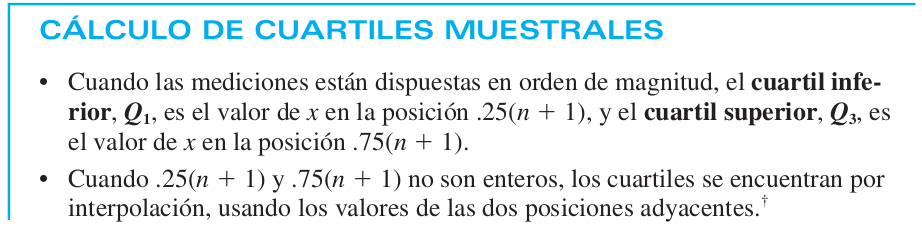
\includegraphics[width=\textwidth]{im27}
\end{center}


\end{frame}
%%%%%%%%%%%%%%%%%%%%%%%%%%%%%%%%%%%%%%%%%%%%%%%%%%%%%%%%%%%%%%%%%%%%%%%%%%%%%%%%%%%%%%%%%%%%%%%%%%%%%%%%%%%%%
\begin{frame}
\frametitle{Cuartil}

\begin{center}
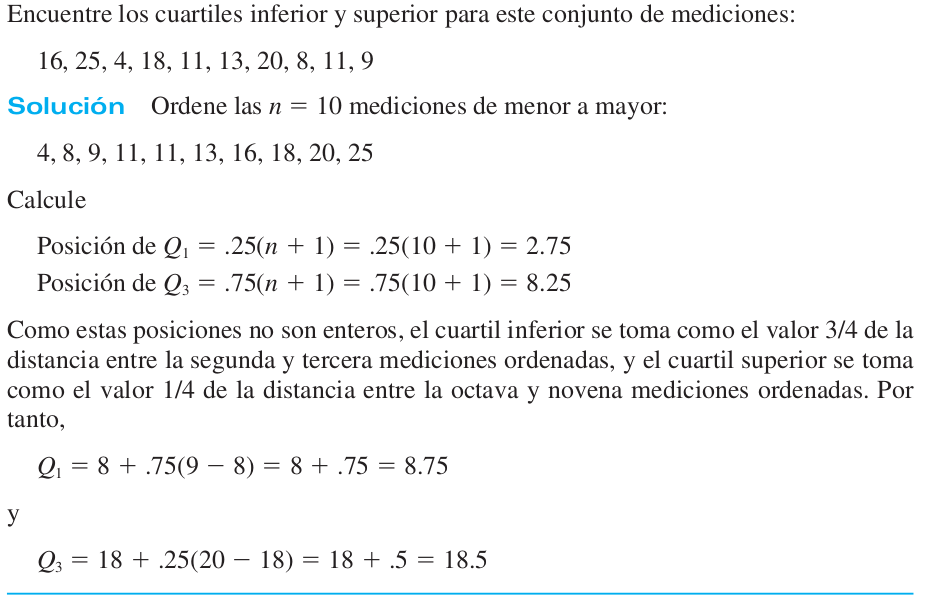
\includegraphics[width=\textwidth]{im28}
\end{center}


\end{frame}
%%%%%%%%%%%%%%%%%%%%%%%%%%%%%%%%%%%%%%%%%%%%%%%%%%%%%%%%%%%%%%%%%%%%%%%%%%%%%%%%%%%%%%%%%%%%%%%%%%%%%%%%%%%%%
\begin{frame}
\frametitle{Intercuartil}
Como la mediana y los cuartiles dividen la distribución de datos en cuatro partes, cada una de ellas conteniendo alrededor de 25\% de las mediciones, $Q_1$ y $Q_3$ son las fronteras superior e inferior para el 50\% central de la distribución. Podemos medir el rango de este “50\% central” de la distribución usando una medida numérica llamada rango intercuartil.

\begin{block}{Definición}
El rango intercuartil (IQR) para un conjunto de mediciones es la diferencia entre los cuartiles superior e inferior; esto es, $IQR = Q_3 - Q_1$ .
\end{block}
\end{frame}
%%%%%%%%%%%%%%%%%%%%%%%%%%%%%%%%%%%%%%%%%%%%%%%%%%%%%%%%%%%%%%%%%%%%%%%%%%%%%%%%%%%%%%%%%%%%%%%%%%%%%%%%%%%%%
\begin{frame}
\frametitle{El resumen de cinco números y la gráfica de caja}


\begin{center}
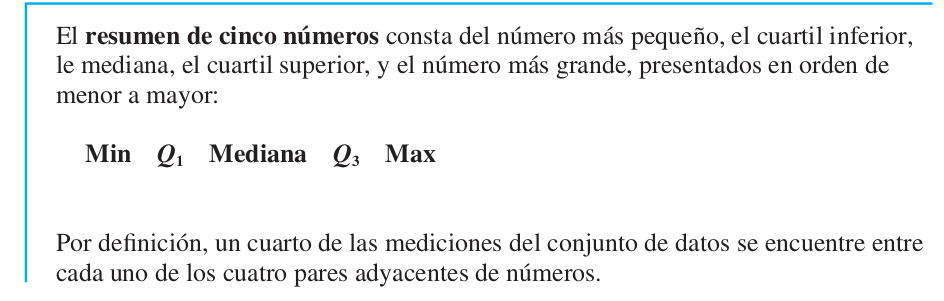
\includegraphics[width=\textwidth]{im29}
\end{center}

\end{frame}
%%%%%%%%%%%%%%%%%%%%%%%%%%%%%%%%%%%%%%%%%%%%%%%%%%%%%%%%%%%%%%%%%%%%%%%%%%%%%%%%%%%%%%%%%%%%%%%%%%%%%%%%%%%%%
\begin{frame}
\frametitle{El resumen de cinco números y la gráfica de caja}


\begin{center}
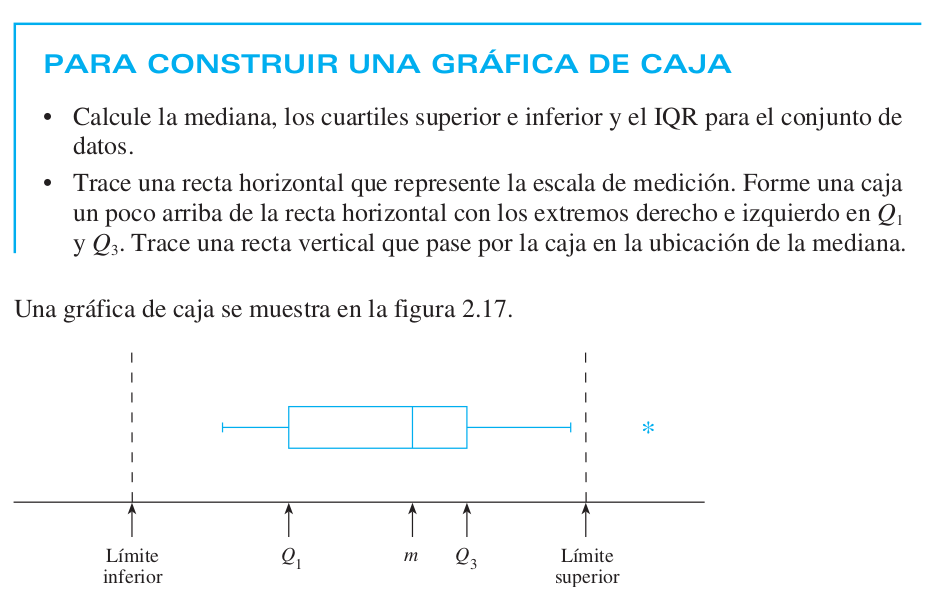
\includegraphics[width=\textwidth]{im30}
\end{center}

\end{frame}
%%%%%%%%%%%%%%%%%%%%%%%%%%%%%%%%%%%%%%%%%%%%%%%%%%%%%%%%%%%%%%%%%%%%%%%%%%%%%%%%%%%%%%%%%%%%%%%%%%%%%%%%%%%%%
\end {document}



                                                  






